\chapter{Implementierung}

Das vorliegende Kapitel widmet sich der umfassenden Dokumentation des Implementierungsprozesses des zuvor beschriebenen
Konzepts. Es bietet eine detaillierte Aufarbeitung der technischen Umsetzung und des Entwicklungsprozesses, der im
Rahmen dieser Masterarbeit durchgeführt wurde. Beginnend mit einer umfassenden Beschreibung der verwendeten Technologien
und Werkzeuge sowie einer ausführlichen Begründung für die Wahl dieser spezifischen Technologien, wird dieses Kapitel
einen tiefen Einblick in die präzise Umsetzung des Konzepts gewähren. Die Implementierung ist ein entscheidender Schritt
zur Realisierung des in den vorherigen Kapiteln skizzierten Ansatzes zur Bewertung von UML-Diagrammen. Durch die
Dokumentation dieses Schrittes wird das Verständnis für die technischen Aspekte des Projekts vertieft und ermöglicht
eine transparente Darstellung des Entwicklungsprozesses.

\section{Überblick über angewendete Werkzeuge und Technologien}
Dieses Kapitel konzentriert sich auf die Vorstellung der Werkzeuge, die für die Umsetzung des im vorherigen Kapitel
vorgestellten Konzepts verwendet werden. Es wird jedes Werkzeug vorgestellt und die Auswahl begründet.

\subsection{PlantText}

Der erste Schritt des im vorherigen Kapitel vorgestellten Konzepts besteht in der Modellierung eines UML-Diagramms.
Diese Modellierungsphase verlangt die Anwendung einer Software-Anwendung, welche in der Lage ist, das entworfene
Diagramm in ein Format zu überführen, welches für die anschließende Extraktion der enthaltenen Regelsätze dienlich
ist. Eine facettenreiche Auswahl an digitalen Werkzeugen steht zur Verfügung, um diese spezifische Aufgabe zu
bewältigen, wobei PlanText exemplarisch zu nennen ist.

PlantText~\cite{planttext} ist ein webbasiertes Instrument zur Diagrammmodellierung, das insbesondere in den Domänen
der UML und anderer Modellierungssprachen einen renommierten Status innehat. Dieses Instrument wurde entwickelt,
um die bequeme Erstellung, Bearbeitung und gemeinsame Nutzung von Diagrammen in einer kollaborativen Umgebung zu
ermöglichen. Seine Auszeichnungen resultieren aus der Benutzerfreundlichkeit, der Flexibilität und der
Leistungsfähigkeit, wodurch es zu einer favorisierten Wahl für Softwareentwickler, Systemarchitekten und Projektmanager
avanciert~\cite{planttext}.

PlantText basiert auf einer schlichten, aber wirkungsvollen Konzeption, nämlich der Generierung von Diagrammen durch
Verwendung von textuellen Notationen. Benutzer können Diagramme unter Einsatz von natürlicher Sprache und vordefinierten
Schlüsselwörtern kreieren, wodurch der gesamte Prozess simplifiziert wird. Eine prototypische Darstellung einer Klasse
in einem UML-Klassendiagramm kann etwa wie folgt aussehen:


\begin{lstlisting}[caption={[Codebeispiel] PlantText code Example}, label={lst:Planttext}, float=!ht, language=javascript]
class A {
   + attribute1: Typ1
   - attribute2: Typ2
   # operation1(): void
}
\end{lstlisting}

In diesem Illustrationsfall repräsentieren einfache Textnotationen die Klasse ``A'', ihre Attribute und Methoden.
Die Verwendung von ``+'' für öffentliche Attribute, ``-'' für private Attribute und ``#'' für Methoden gestaltet sich
intuitionsgetreu und erleichtert die Entwicklung von UML-Diagrammen erheblich. PlantText beinhaltet eine leistungsstarke
Rendering-Engine, die diese textlichen Notationen automatisiert in visuell ansprechende Diagramme konvertiert. Benutzer
sind in der Lage, die Diagramme in Echtzeit zu visualisieren und zu editieren, ohne sich mit den komplexen Details der
grafischen Gestaltung auseinandersetzen zu müssen. Diese textorientierte Herangehensweise führt zu einer höchst
effizienten und adaptierbaren Gestaltung und Veränderung von Diagrammen. Die Vorzüge der Anwendung von PlantText
manifestieren sich unter anderem in:

\begin{enumerate}
    \item \textbf{Benutzerfreundlichkeit:} PlantText ist für Einsteiger und erfahrene Modellierer gleichermaßen zugänglich.
Die Verwendung von textuellen Notationen vereinfacht den Einstieg und reduziert die Lernkurve, da sie natürlicher und
verständlicher sind als grafische Schnittstellen.
    \item \textbf{Kollaboration und gemeinsame Nutzung:} PlantText bietet eine eingebettete Kollaborationsplattform, auf
der mehrere Benutzer simultan an Diagrammen arbeiten können. Dies fördert die Teamarbeit und erlaubt die
Echtzeit-Erstellung und Überarbeitung von Modellen.
    \item \textbf{Plattformunabhängigkeit:} Da PlantText webbasiert ist, ist es plattformneutral. Benutzer können von
jedem Gerät mit Internetzugang auf ihre Modelle zugreifen und sie editieren, ohne Softwareinstallationen durchführen
zu müssen.
    \item \textbf{Erweiterbarkeit:} PlantText unterstützt nicht ausschließlich UML, sondern auch diverse andere
Modellierungssprachen und Diagrammtypen. Infolgedessen entwickelt sich PlantText zu einem vielseitigen Werkzeug für eine
Vielzahl von Anwendungsszenarien.
\end{enumerate}

\begin{figure}
    \centering
    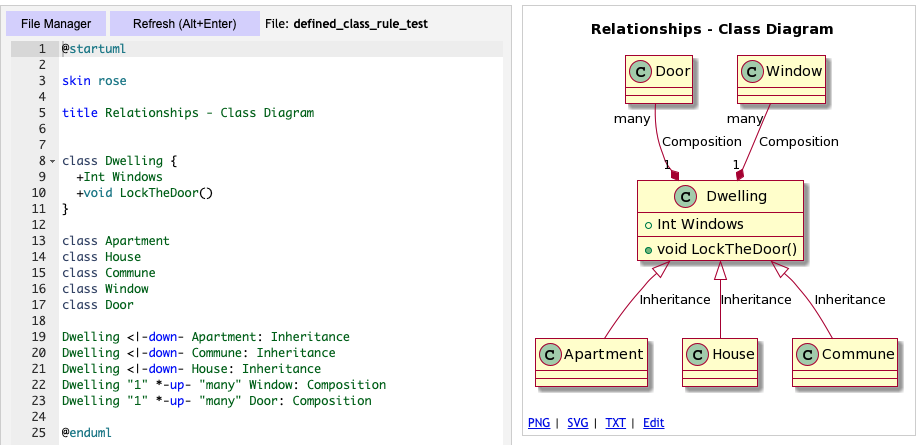
\includegraphics[width=15cm]{images/plantText.png}
    \caption{Grafische Benutzeroberfläche von plantText}
    \label{fig:plant-text}
\end{figure}

Vor der Wahl von PlantText als Instrument für die Entwurfsphase der Anwendung wurden mehrere Modellierungswerkzeuge
einer eingehenden Prüfung unterzogen. Diese Werkzeuge schlossen namhafte Anwendungen wie Enterprise Architect~\cite{enterarch},
Astah UML~\cite{astah}, MagicDraw~\cite{magic}, Visual Paradigm~\cite{visual}, Umbrello \cite{umbrello} und Draw.io \cite{draw} ein.
Eine gemeinsame Eigenschaft dieser Werkzeuge besteht darin, dass sie sich für die rasche Erstellung von Diagrammen
eignen, was auf ihre intuitive Benutzeroberfläche, leichte Verständlichkeit und Nutzerfreundlichkeit zurückzuführen ist.
Bedauerlicherweise wiesen sie jedoch einen bedeutenden Mangel auf, der ihre Anwendbarkeit in Bezug auf unsere
spezifischen Anforderungen einschränkte. Keines dieser Programme bot die Möglichkeit, die erstellten Diagramme in eine
leicht interpretierbare textuelle Form zu überführen.

Die meisten dieser Tools gestatten zwar das Exportieren der erstellten Diagramme im XML-Format, doch dieses Format
präsentiert lediglich eine räumliche Repräsentation der verschiedenen Objekte in einer Ebene, ohne eine semantische
Tiefenstruktur. Ein weiteres Hindernis bestand darin, dass die Informationen bezüglich der Verbindungen zwischen den
diversen UML-Objekten nur mit großem Aufwand und erheblichen Schwierigkeiten aus dem generierten XML extrahiert werden
konnten. Dies wäre in der Praxis äußerst zeitaufwendig und würde die Entwicklung eines eigenen Parsers erfordern, um die
relevanten Informationen zu extrahieren und in eine verwertbare Form zu überführen.

Die Nutzung von PlantText hingegen bietet einen klaren Vorteil in dieser Hinsicht. Dies resultiert aus der bereits
implementierten PlantUML-Engine, die über einen eingebauten Parser verfügt. Diese Funktionalität ermöglicht es,
den erstellten Code direkt in einem Format zu erhalten, das für die Weiterverarbeitung und Interpretation äußerst zugänglich ist.
Diese grundlegende Unterscheidung führt dazu, dass PlantText in unserem Anwendungsfall als überlegen angesehen wird.
Durch die Fähigkeit zur Bereitstellung des Modells in einer textuellen Form ermöglicht es eine tiefere und
bedeutungsvollere Analyse der erstellten Diagramme. Dies fördert die Genauigkeit bei der Modellierung und stellt sicher,
dass die erstellten Diagramme nicht nur als visuelle Darstellungen betrachtet werden, sondern auch als Quellen
semantischer Informationen dienen können.

\subsection{PlantUML + Nodejs}


\subsection{Vue.js}

\section{Darlegung des Workflow-Prozesses}

\section{Einrichtung und Entwicklung des ``GReQL Converter''}